	\documentclass[12pt,spanish]{article}
	\usepackage{graphicx}
	\graphicspath{ {Graficas/}}
	\usepackage[T1]{fontenc}
	\usepackage[utf8]{inputenc}
	\usepackage{pdfpages}
	\usepackage{hyperref}
	
	\usepackage{fancyhdr}
	\usepackage{amssymb}
	\usepackage{amsmath}
	\usepackage{enumerate}
	\usepackage[noend]{algpseudocode}
	\usepackage{algorithm}
	\usepackage[spanish]{babel}
	\usepackage{vmargin}
	\usepackage{subcaption}
	\setpapersize{A4}
	\setmargins{2cm}       % margen izquierdo
	{1.5cm}                % margen superior
	{16.5cm}               % anchura del texto
	{23.42cm}              % altura del texto
	{10pt}                 % altura de los encabezados
	{1cm}                  % espacio entre el texto y los encabezados
	{0pt}                  % altura del pie de página
	{2cm}                  % espacio entre el texto y el pie de página
	
	\providecommand{\abs}[1]{\lvert#1\rvert}
	\pagestyle{fancy}
	\newcommand{\sectionbreak}{\clearpage}
	
	\usepackage{xcolor}
	\hypersetup{
		colorlinks,
		linkcolor={black!50!black},
		citecolor={blue!50!black},
		urlcolor={blue!80!black}
	}
	\rhead{Practica 3}
	\lhead{Criptografía y Computación}
	
	\setcounter{secnumdepth}{0} % sections are level 1
	
	\author{
		\\\\
		
\includegraphics[scale=1]{UGR} \\
		\linebreak\\
		\Large Rafa Bailón Robles\\
		\Large Antonio Manuel Fresneda Rodríguez\\
		\Large Ismael Marín Molina\\
	}

	\title{\huge \textbf{Criptografía y Computación\\ Práctica 3}}

    \begin{document}
        \maketitle
        \pagebreak
        \tableofcontents
        \pagebreak
 	\section{Logaritmo Discreto}
	\subsection{Explicación}
	 	El objetivo en esta sección es el de resolver el problema del logaritmo discreto y ver como se comportan distintos algoritmos cuando el problema crece:\\
	 	Dados un primo $p$, $a$ un entero tal que $2 \leq a \leq p-2$ y $b$ otro entero $1 \leq b \leq p-1$ encontrar $x$ tal que $a^{x} \equiv b \pmod{p}$.\\
	 	Se han usado los siguientes algoritmos: 
	 	\begin{itemize}
	 		\item\textbf{Fuerza bruta}.
	 		\item\textbf{Paso enano - paso gigante}.
	 		\item\textbf{Rho de Pollard}.
	 	\end{itemize}
		En cuanto a la ejecución de los algoritmos, se han establecido un número de iteraciones para cada uno de los algoritmos y en cada una se incrementa en dos bits el primo en el que se está trabajando. El primer primo de cada iteración tiene 5 bits.
		\pagebreak
	\subsection{Gráficas}
		A continuación se presentan unas graficas en las que vemos como crece el problema cuando vamos aumentando la dificultad: 
		\begin{figure}[!htbp]
			
			\begin{subfigure}{.5\textwidth}
				\centering
				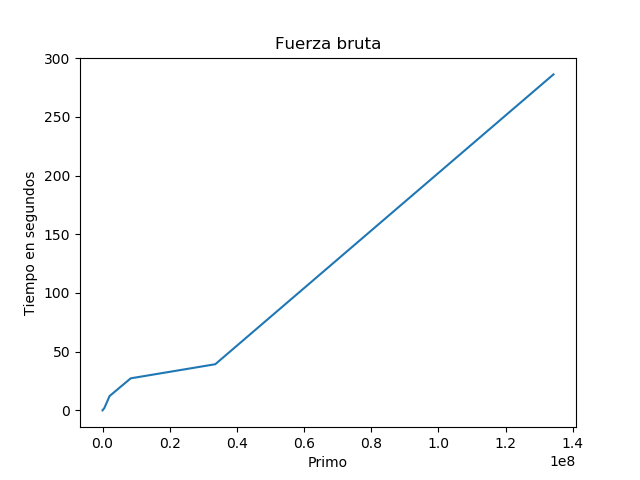
\includegraphics[width=.8\linewidth]{log_bf}
				\caption{Usando el algoritmo de fuerza bruta.}
				\label{fig:sfig11}
			\end{subfigure}%
			\begin{subfigure}{.5\textwidth}
				\centering
				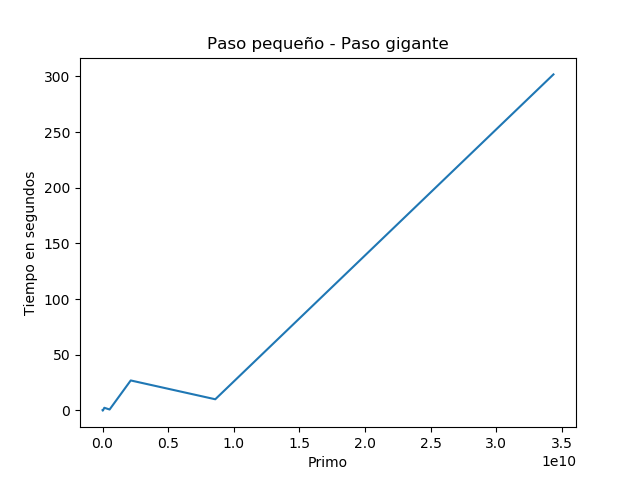
\includegraphics[width=.8\linewidth]{log_pe}
				\caption{Usando el algoritmo de paso enano - paso gigante.}
				\label{fig:sfig12}
			\end{subfigure}
			\begin{subfigure}{.5\textwidth}
				\centering
				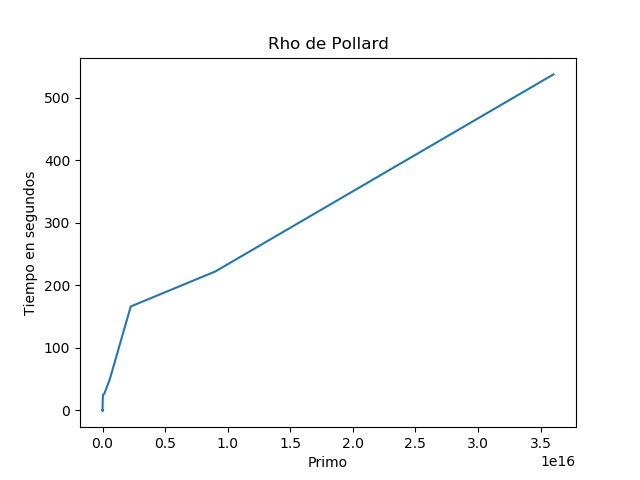
\includegraphics[width=.8\linewidth]{log_ro}
				\caption{Usando el algoritmo Rho de Pollard.}
				\label{fig:sfig13}
			\end{subfigure}
		\caption{Graficas logaritmo discreto.}
		\label{fig:fig1}
		\end{figure}
	\subsection{Conclusiones}
	Observando las gráficas anteriores, vemos como los distintos algoritmos que hemos usado llega un momento en el que tiempo empleado en resolver el problema se dispara.\\
	Si comparamos los tres algoritmos vemos como el de fuerza bruta ha sido el que peor se ha comportado, seguido del algoritmo de paso enano - paso gigante y el algoritmo que mejor se ha comportado ha sido el de Rho de Pollard.\\
	\end{document}